\documentclass[12pt]{article}
\usepackage[top=1in, bottom=1in, left=1in, right=1in]{geometry}
\parindent 22pt

\usepackage{adjustbox}
\usepackage{amsmath}
\usepackage{amssymb}
\usepackage{array}
\usepackage{booktabs}
\usepackage{datetime}
\usepackage{fancyhdr}
\usepackage{float}
\usepackage{graphicx}
\usepackage[colorlinks=true,linkcolor=blue,urlcolor=blue,anchorcolor=blue,citecolor=blue]{hyperref}
\usepackage{lscape}
\usepackage{multirow}
\usepackage{natbib}
\usepackage{setspace}
\usepackage{tabularx}
\usepackage[colorinlistoftodos,linecolor=black]{todonotes}
\usepackage{appendix}
\usepackage{pgffor}
\usepackage{caption} 
\usepackage{threeparttable}
\captionsetup[table]{skip=3pt}

\settimeformat{hhmmsstime}

\newcolumntype{L}[1]{>{\raggedright\arraybackslash}p{#1}}
\newcolumntype{C}[1]{>{\centering\arraybackslash}p{#1}}
\newcolumntype{R}[1]{>{\raggedleft\arraybackslash}p{#1}}


\begin{document}

\doublespacing

\subsection{Differences in parents' education}

Figures \ref{fig:momEdu} and \ref{fig:dadEdu} presents the distribution of parental educational attainment for individuals from each materna type-city-cohort combination. Figure \ref{fig:momEdu} shows that within Reggio, mothers of individuals who did not attend preschool have proportionally higher levels of high school and university education than mothers of individuals who attended some form of preschool. This difference is more pronounced for the older cohorts. Figure \ref{fig:dadEdu} shows a similar pattern persists when examining father's education. A clear pattern does not emerge when we compare parental educational attainment between individuals who attended preschool in Reggio. This suggests that parental education might have played a larger role in the initial decision of sending an individual to preschool, as compared to the subsequent decision of choosing a particular type of preschool. Figures \ref{fig:momEdu} and \ref{fig:dadEdu} include analogous graphs for Parma and Padova.

Figure \ref{fig:parentsEdu} examines inequality of educational attainment between mothers and fathers for individuals from each city-cohort combination. Each column represents the total proportion of individuals in each city-cohort combination whose fathers are more educated than mothers. Each column is further broken down into sections that calculate this proportion conditional on different levels of father's education. The figures show that total inequality in educational attainment is largest in Padova and smallest in Reggio, and that this ranking of total inequality is consistent across the three adult cohorts. Furthermore, for the older cohorts, the level of inequality is substantially larger in Padova compared to Reggio and Parma. Padova begins to look similar to the other two cities by the time we reach the age 30 cohort. 


\begin{figure}[!htb]
	\begin{minipage}{1\textwidth}
	\centering
	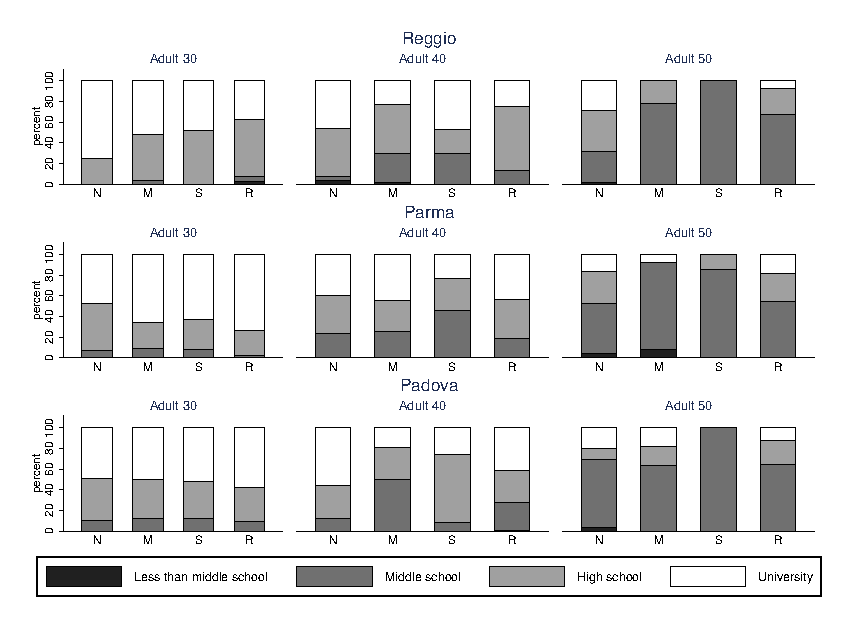
\includegraphics[scale=1.2]{../../../../Output/image/bar_momEdu}
	\caption{Mother's education by city, cohort and materna type}
	\label{fig:momEdu}
	\footnotetext{\textbf{Note:  (1)} Definiteion of bar labels: N = Not attended; M = Municipal; S = State; R = Religious. \textbf{(2)} Each bar presents the distribution of mothers' educational attainment for individuals in each city-cohort-materna type combination. }
	\end{minipage}
\end{figure}

\begin{figure}[!htb]
	\begin{minipage}{1\textwidth}
	\centering
	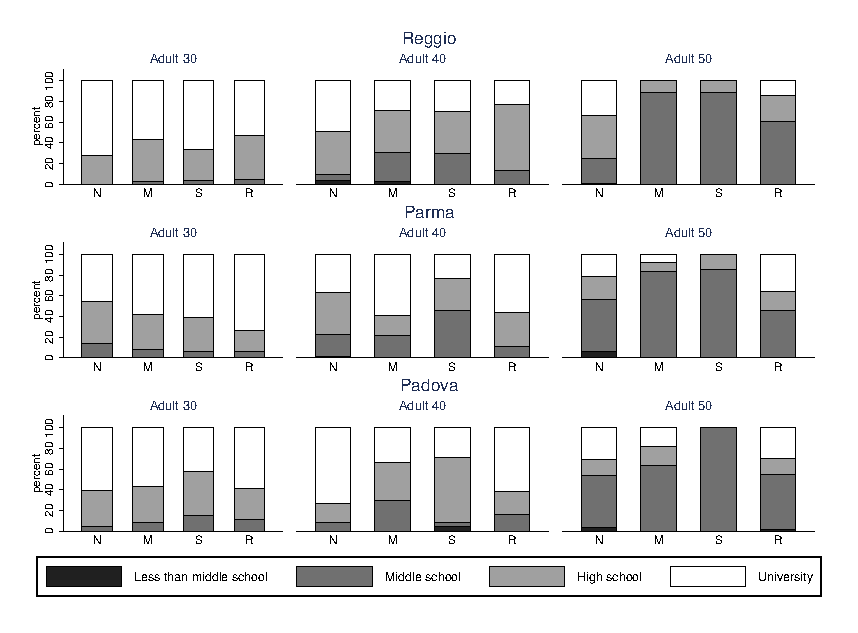
\includegraphics[scale=1.2]{../../../../Output/image/bar_dadEdu}
	\caption{Father's education by city, cohort and materna type}
	\label{fig:dadEdu}
	\footnotetext{\textbf{Note:  (1)} Definiteion of bar labels: N = Not attended; M = Municipal; S = State; R = Religious. \textbf{(2)} Each bar presents the distribution of fathers' educational attainment for individuals in each city-cohort-materna type combination. }
	\end{minipage}
\end{figure}

\begin{figure}[!htb]
	\begin{minipage}{.9\textwidth}
	\centering
	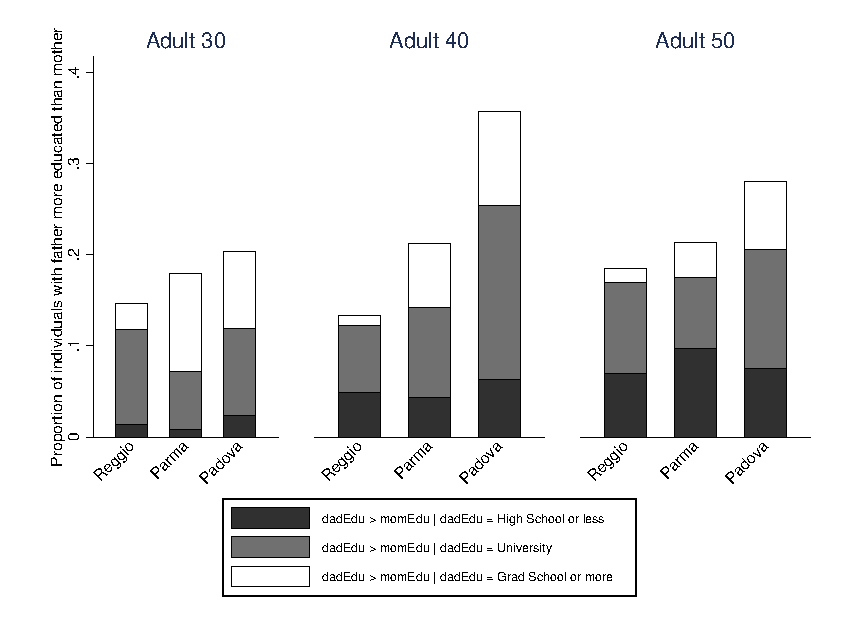
\includegraphics[scale=1]{../../../../Output/image/bar_parentsEduCompare}
	\caption{Proportion of individuals with fathers who are more educated than mothers by city and cohort}
	\label{fig:parentsEdu}
	\footnotetext{\noindent \textbf{Note:   } Each column represents the proportion of individuals within each city-cohort combination whose fathers were more educated than their mothers.}
	\end{minipage}
\end{figure}


\end{document}
